\documentclass{article}

\textwidth=6.5in
\textheight=8.5in
\voffset=-54pt
\oddsidemargin=0in
\evensidemargin=0in
\setlength{\parskip}{8pt}
\setlength{\parindent}{0pt}

\usepackage{amsmath, amssymb}
\usepackage{ifthen}

\usepackage[inline]{enumitem}
\setlist{topsep=0pt, parsep=8pt}

\usepackage[rgb,table]{xcolor}\convertcolorsUfalse
\usepackage{graphicx}

% change hyperref options
\PassOptionsToPackage{hyphens}{url}
\usepackage[bookmarks,colorlinks,linkcolor=black,citecolor=blue,pdfstartview=FitH,urlcolor=blue]{hyperref}
\hypersetup{pdfpagemode=UseNone}
\usepackage{bookmark}

\usepackage{graphicx}
\usepackage{multicol}
\usepackage{framed}
\usepackage{array}

\usepackage{icomma}

\usepackage{soul}
\usepackage[normalem]{ulem}

\usepackage{pgfplots}
\pgfplotsset{compat=1.18}  
\pgfplotscreateplotcyclelist{mycolor}{black, blue, red, green!70!black, magenta, purple, cyan, orange }  
\pgfplotsset{
  disabledatascaling,
  cycle list=tikzcolor, 
  axis lines=middle,
  every axis plot/.style={no marks, thick},
  every axis/.style={
    enlarge x limits=false,
    enlarge y limits=auto,
    xlabel style={at={(current axis.right of origin)},anchor=west},
    ylabel style={at={(current axis.above origin)},anchor=south},
    % extra x and y ticks for asymptotes
    extra x tick style={grid=major, grid style={dashed,black}},
    extra y tick style={grid=major, grid style={dashed,black}},
    /pgf/number format/1000 sep={},
  },    
  tick label style = {font=\footnotesize, fill=\currentbgcolor, inner sep=0pt},    
  xticklabel shift=1pt,    
  scaled ticks=false,
  scaled y ticks=false,
  unbounded coords=jump,
  samples=101,
  minor tick length=0,
  scatter/classes={
    open={mark=*,draw=black,fill=white, mark size=2, thin},
    closed={mark=*,draw=black,fill=black, mark size=2, thin}
  },
  width=3in,
}
\pgfplotsset{open/.style={only marks, mark=*, fill=white, thin, mark size=2}}
\pgfplotsset{closed/.style={only marks, mark=*, draw=black, fill=black,
    thin, mark size=2}}
\pgfplotsset{labeled/.style={nodes near coords, only marks, mark=*, draw=black, fill=black, thin, mark size=2, point meta=explicit symbolic}}

\usepackage{tikz}
\usetikzlibrary{
  matrix,%
  % enables the snake paths
  decorations.pathmorphing,%
  % enables bigger arrows
  decorations.markings,%
  decorations.pathreplacing,%
  decorations.text,%
  calc,%
  patterns,%
  shapes.geometric,%
  arrows,
  decorations.shapes,
  positioning,
  plotmarks,
  intersections
}
\tikzset{>=latex} % sets default arrow type in tikz
\tikzset{font=\normalsize}
\tikzset{mark size=1.5pt, mark options=thin}
\tikzset{pin distance=4pt,
  every pin edge/.style={<-, thin, shorten <= -2pt}}

\interfootnotelinepenalty=10000
\renewcommand{\thefootnote}{(\arabic{footnote})}

\usepackage{multirow, bigdelim}

% change to \usepackage[sols]{handout} to see solutions
\usepackage[]{handout}

\newcommand\iscurrentenumi[1]{%
  \ifthenelse{\equal{#1}{\theenumi}}{}{#1}}
\setenumerate[1]{ref=\#\arabic*}
\setenumerate[2]{ref=\protect\iscurrentenumi{\theenumi}(\alph*)}
\newcommand\enumiiprefix[2]{%
  \ifthenelse{{\equal{#1}{\theenumi}}\AND{\equal{#2}{(\alph{enumii})}}}{}{}%
  \ifthenelse{{\equal{#1}{\theenumi}}\AND{\NOT{\equal{#2}{(\alph{enumii})}}}}{#2}{}%
  \ifthenelse{\equal{#1}{\theenumi}}{}{#1#2}%
}
\setenumerate[3]{ref=\protect\enumiiprefix{\theenumi}{(\alph{enumii})}\roman*}

\newlength{\tipmargin}
\makeatletter

\renewenvironment{framed}{
  \setlength{\tipmargin}{\textwidth-\linewidth}
  \advance\@totalleftmargin-\tipmargin
  \def\FrameCommand{\hspace{\tipmargin}\fbox}%
  \advance\linewidth\tipmargin
  \MakeFramed {\advance\hsize-\width \FrameRestore}%
}
{\endMakeFramed}

\makeatother

\definecolor{purple}{rgb}{0.5,0,1.0}

\usepackage{fancyhdr}
\lhead{\textcolor{white}{This content is protected and may not be shared, uploaded, or distributed.}}
\rhead{}
\rfoot{\vspace*{\fill}\footnotesize\textcopyright{} \emph{Harvard Math Ma}}
\renewcommand{\headrulewidth}{0pt}
\pagestyle{fancy}
\begin{document}

\htitle{More Differentiation Rules, Tangent Line Approximation}

\begin{problemonly}
  \begin{framed}

You should be able to:
    \begin{itemize}[topsep=0pt,partopsep=0pt,parsep=8pt,itemsep=0pt]
    \item Explain why the Product and Quotient Rule are true, and use them (together with the rules we've learned before) to differentiate functions.

    \item Identify functions that can and can't be differentiated using just the rules we've learned so far.

    \item Use secant lines and tangent lines to approximate values like $\sqrt{22}$, and use concavity to determine whether your approximations are upper or lower bounds. 

    \end{itemize}
  \end{framed}
\end{problemonly}

\begin{enumerate}
\item  \label{beanstalk-recap} (\href{https://people.math.harvard.edu/~jjchen/mathma/docs/homework/PS17.html}{Problem Set 17}, {{\#5}}) 

  \note{This is setting students up for \ref{product-rule-lengths}.}

  \begin{problem}[0.75in]
    At noon one day, Jack plants a magical bean. To his delight, it grows quickly into a giant beanstalk. Let $f(t)$ be the beanstalk's height in feet $t$ hours after noon.

    If $h$ is a fairly small positive number, roughly how much does the beanstalk grow between $t$ hours after noon and $t + h$ hours after noon? 
  \end{problem}

  \begin{solution}
    See \href{https://people.math.harvard.edu/~jjchen/mathma/docs/homework/PS17.html}{Problem Set 17}, {{\#5}}. 
  \end{solution}

\item  Suppose we have two differentiable functions $f$ and $g$, and let $P(t) = f(t) g(t)$ be their product.
  \begin{enumerate}
  \item \label{product-rule-limit-def}
    \begin{problem}[0.75in]
      According to the limit definition of the derivative, what is $P'(t)$?
    \end{problem}

    \begin{solution}
      \begin{align*}
        P'(t) &= \lim_{h \to 0} \frac{P(t+h)-P(t)}{h} \\
        &=  \lim_{h \to 0} \frac{f(t+h)g(t+h)-f(t)g(t)}{h}
      \end{align*}
    \end{solution}

  \item
    \begin{problem}[\vfill\newpage]
      Can you think of a picture to draw to represent a product?
    \end{problem}

    \begin{solution}
      We can represent the product of two numbers $a$ and $b$ 
      as the area of a rectangle with side
      lengths $a$ and $b$.
    \end{solution}

  \item

    \note{GeoGebra for a rectangle where you can grab a corner and make it grow: \url{https://www.geogebra.org/m/wswuwdbt}} 

    Imagine a rectangle that's growing over time. Let $f(t)$ and $g(t)$ be its height and width at time $t$. Imagine looking at the rectangle at time $t$:

    \begin{tikzpicture}[x=1in, y=1in]
      \newcommand{\currentcolor}{white}
      \coordinate (X) at (2, 0); %
      \coordinate (Y) at (0, 1); %
      \coordinate (growX) at (2.5, 0); \coordinate (growY) at (0, 1.4);
      \coordinate (info) at (3, 3); %
      \begin{scope}[\currentcolor]
        \draw[ultra thick] (0, 0) -- (growX) -- (growX |- Y) -- (Y) -- (0, 0); %
        \draw[|-|] (-60pt, 0) -- node[fill=white]{$f(t + h)$} ($(Y) - (60pt, 0)$); %
      \end{scope}
      \draw[thin] (0, 0) -- (X) -- (X |- Y) -- (Y) -- (0, 0); %
      \draw[|-|] (0, -12pt) -- node[fill=white]{$g(t)$} ($(X) - (0, 12pt)$); %
      \draw[|-|] (-16pt, 0) -- node[fill=white]{$f(t)$} ($(Y) - (16pt, 0)$); %
    \end{tikzpicture}

    and then again a short time later, at time $t + h$:

    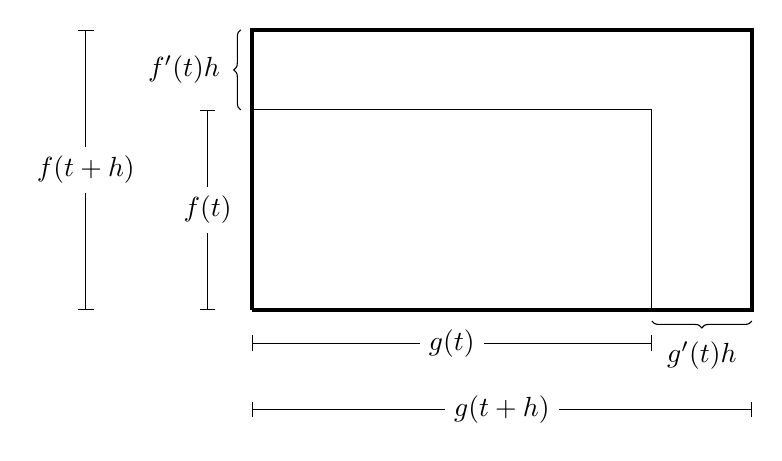
\begin{tikzpicture}[x=1in, y=1in]
      \newcommand{\currentcolor}{black}
      \coordinate (X) at (2, 0); %
      \coordinate (Y) at (0, 1); %
      \coordinate (growX) at (2.5, 0); %
      \coordinate (growY) at (0, 1.4); %
      \coordinate (info) at (3, 3); %
      \begin{scope}[\currentcolor]
        \draw[ultra thick] (0, 0) -- (growX) -- (growX |- growY) -- (growY) -- (0, 0); %
        \draw[|-|] (0, -36pt) -- node[fill=white]{$g(t + h)$} ($(growX) - (0, 36pt)$); %
        \draw[|-|] (-60pt, 0) -- node[fill=white]{$f(t + h)$} ($(growY) - (60pt, 0)$); %
      \end{scope}
      \draw[thin] (0, 0) -- (X) -- (X |- Y) -- (Y) -- (0, 0); %
      \draw[|-|] (0, -12pt) -- node[fill=white]{$g(t)$} ($(X) - (0, 12pt)$); %
      \draw[|-|] (-16pt, 0) -- node[fill=white]{$f(t)$} ($(Y) - (16pt, 0)$); %
      \draw[decorate, decoration={brace, mirror}] ($(growY) - (4pt, 0)$) -- node[left, xshift=-4pt]{\solonly{$f'(t)h$}} ($(Y) - (4pt, 0)$); %
      \draw[decorate, decoration={brace}] ($(growX) - (0, 4pt)$) -- node[below, yshift=-4pt]{\solonly{$g'(t)h$}} ($(X) - (0, 4pt)$);%
    \end{tikzpicture}

    \begin{enumerate}
    \item \label{product-rule-lengths}

      \begin{problem}[0.5in]
        Approximate the lengths marked by the braces. (Hint: How is \ref{beanstalk-recap} relevant?) 
      \end{problem}

      \begin{solution}
        Since the lengths marked by the braces are the change from $f(t)$ to $f(t+h)$ and
        the change from $g(t)$ to $g(t+h)$, we can approximate them as $f'(t)h$ and $g'(t)h$
        respectively.
      \end{solution}

    \item
      \begin{problem}[\vfill]
        How would you picture $P(t + h)$ in this picture? How about $P(t)$? Use this to find $P'(t)$.
      \end{problem}

      \begin{solution}
        In this picture, $P(t+h)$ is the area of the bigger rectangle whose sides are $f(t+h)$
        and $g(t+h)$, while $P(t)$ is the area of the smaller rectangle whose
        sides are $f(t)$ and $g(t)$. 

        We can divide the larger rectangle up into four smaller rectangles like this.
        
    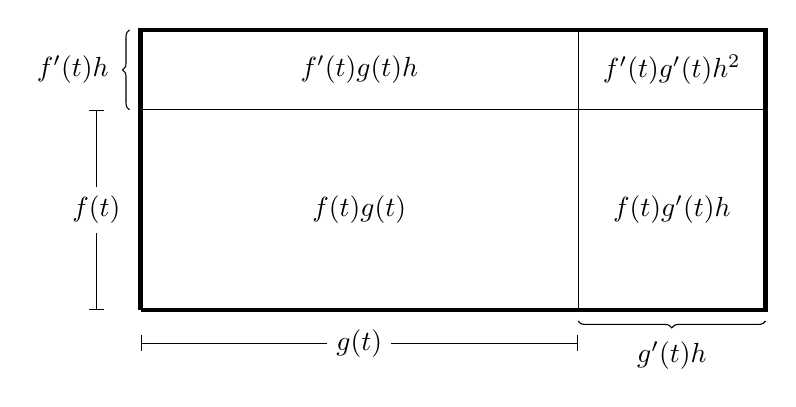
\begin{tikzpicture}[x=1.25in, y=1in]
      \newcommand{\currentcolor}{black}
      \coordinate (X) at (1.75, 0); %
      \coordinate (Y) at (0, 1); %
      \coordinate (growX) at (2.5, 0); %
      \coordinate (growY) at (0, 1.4); %
      \coordinate (info) at (3, 3); %
      \begin{scope}[\currentcolor]
        \draw[ultra thick] (0, 0) -- (growX) -- (growX |- growY) -- (growY) -- (0, 0); %
      \end{scope}
      \draw[thin] (X) -- (X |- growY); %
      \draw[thin] (Y) -- (Y -| growX); %
      \draw[|-|] (0, -12pt) -- node[fill=white]{$g(t)$} ($(X) - (0, 12pt)$); %
      \draw[|-|] (-16pt, 0) -- node[fill=white]{$f(t)$} ($(Y) - (16pt, 0)$); %
      \draw[decorate, decoration={brace, mirror}] ($(growY) - (4pt, 0)$) -- node[left, xshift=-4pt]{\solonly{$f'(t)h$}} ($(Y) - (4pt, 0)$); %
      \draw[decorate, decoration={brace}] ($(growX) - (0, 4pt)$) -- node[below, yshift=-4pt]{\solonly{$g'(t)h$}} ($(X) - (0, 4pt)$);%
      \node at (0.875, 0.5) {$f(t)g(t)$};
      \node at (0.875, 1.2) {$f'(t)g(t)h$};
      \node at (2.125, 0.5) {$f(t)g'(t)h$};
      \node at (2.125, 1.2) {$f'(t)g'(t)h^2$};
    \end{tikzpicture}

        This means that $P(t+h) \approx f(t)g(t) + f'(t)g(t)h + f(t)g'(t)h + f'(t)g'(t)h^2$.
        Let's substitute this into the limit we wrote for $P'(t)$. 
        \begin{align*}
        P'(t) &= \lim_{h \to 0} \frac{P(t+h)-P(t)}{h} \\
        &=  \lim_{h \to 0} \frac{f(t+h)g(t+h)-f(t)g(t)}{h} \\
        &= \lim_{h \to 0} 
        \frac{f(t)g(t) + f'(t)g(t)h + f(t)g'(t)h + f'(t)g'(t)h^2 - f(t)g(t)}{h} \\
        &= \lim_{h \to 0} \frac{f'(t)g(t)h + f(t)g'(t)h + f'(t)g'(t)h^2}{h} \\
        &= \lim_{h \to 0} (f'(t)g(t) + f(t)g'(t) + f'(t)g'(t)h) \\
        &= f'(t)g(t) + f(t)g'(t).
      \end{align*}
      \end{solution}
    \end{enumerate}

  \end{enumerate}

\end{enumerate}
\begin{framed}
  \textbf{Product Rule:} $\displaystyle \frac{d}{dx} [f(x) \cdot g(x)] = 
  \solonly{f'(x) g(x) + f(x)g'(x)}$
\end{framed}

\pspace{\newpage}

\begin{enumerate}[resume, topsep=0pt]
\item 
  \begin{problem}[\vfill]
    Evaluate $\displaystyle \frac{d}{dx} \left[(x^4 + x^7) (3x^7 + x^2) \right]$.
  \end{problem}

  \begin{solution}
    Since we want to find the derivative of the product of two functions, we can use the
    Product Rule. First, let's write down the form of the Product Rule.
    \begin{align*}
      \frac{d}{dx} \left[(x^4 + x^7) (3x^7 + x^2) \right] &=
      \left[\frac{d}{dx} (x^4 + x^7)\right] (3x^7 + x^2) + 
      (x^4 + x^7) \left[\frac{d}{dx} (3x^7 + x^2)\right] \\
      \intertext{Now we can find the derivatives we need using the Power Rule.}
      \frac{d}{dx} \left[(x^4 + x^7) (3x^7 + x^2) \right] 
      &= (4x^3+7x^6)(3x^7 + x^2) + (x^4 + x^7)(21x^6 + 2x).
    \end{align*}
  \end{solution}

\end{enumerate}
\begin{framed}
  \textbf{Quotient Rule} (\emph{you'll show this on homework!}): $\displaystyle \frac{d}{dx} \left( \frac{f(x)}{g(x)} \right) = \frac{g(x) f'(x) - f(x)g'(x)}{g(x)^2}$

  \emph{A way to remember it:} \url{https://youtu.be/jwuiVb84Xx4}
\end{framed}

\begin{enumerate}[resume, topsep=0pt]
\item 
  \begin{problem}[\vfill]
    If $\displaystyle u(r) = \frac{5r + 3}{2r^7 + 1}$, find $\dfrac{du}{dr}$. 
  \end{problem}

  \begin{solution}
    First, let's write down the form of the Quotient Rule.
    \begin{align*}
        \frac{du}{dr} &= \frac{\left[\frac{d}{dr}(5r + 3)\right](2r^7 + 1)
        - (5r + 3)\left[\frac{d}{dr}(2r^7 + 1)\right]}{(2r^7 + 1)^2}\\
        \intertext{Now we can use the Power Rule to find the derivatives we need.}
       \frac{du}{dr} &= \frac{(5)(2r^7 + 1)
        - (5r + 3)(14r^6)}{(2r^7 + 1)^2}.
    \end{align*}
  \end{solution}

\item  \emph{Practice!} Find the derivative of each function \uline{without} using the Quotient Rule. (There are lots of notations for finding derivatives; this problem shows you several.) 

  \begin{enumerate}
  \item
    \begin{problem}[\vfill]
      If $\displaystyle y = \left( \frac{1}{x} - 7x + 4 \right) (x^3 - x + 3)$, find $y'$. 
    \end{problem}

    \begin{solution}
      We can use the Product Rule. First, let's write down the form of the Product Rule.
      \begin{align*}
        y' &= (x^{-1} - 7x + 4)'(x^3 - x + 3) + (x^{-1} - 7x + 4)(x^3 - x + 3)' \\
        \intertext{Now we can find the derivatives we need using the Power Rule.}
        y' &= (-x^{-2} - 7)(x^3 - x + 3) + (x^{-1} - 7x + 4)(3x^2 - 1)
      \end{align*}
    \end{solution}

  \item
    \begin{problem}[\vfill]
      If $\displaystyle y= \frac{7t^2 + 3t + 15}{t \sqrt{t}}$, find $\dfrac{dy}{dt}$.
    \end{problem}

    \begin{solution}
      To do this without using the Quotient Rule, we can first rewrite the function
      using algebra.
      \begin{align*}
        y &= \frac{7t^2 + 3t + 15}{t \sqrt{t}} \\
        &= \frac{7t^2 + 3t + 15}{t^{3/2}} \\
        &= 7t^{1/2} + 3t^{-1/2} + 15t^{-3/2}. \\
        \intertext{Now we can use the Power Rule.}
        \frac{dy}{dt} &= 7(\tfrac{1}{2}t^{-1/2}) + 3(-\tfrac{1}{2}t^{-3/2}) + 
        15(-\tfrac{3}{2}t^{-5/2}) \\
        \intertext{We can optionally simplify by factoring out $\frac{1}{2}t^{-5/2}$.}
        \frac{dy}{dt} &=\tfrac{1}{2}t^{-5/2}(7t^2 -3t -45) \\
        &= \frac{7t^2 -3t -45}{2\sqrt{t^5}}.
      \end{align*}
    \end{solution}

  \item
    \begin{problem}[\vfill]
      If $\displaystyle h(w) = \frac{5w^2 + 4w + 3}{\pi}$, find $h'(w)$. 
    \end{problem}

    \begin{solution}
      To do this without using the Quotient Rule, we can rewrite $h(w)$ as
      $h(w) = \frac{1}{\pi}(5w^2 + 4w + 3)$. This lets us use the Constant Multiple Rule.
      \begin{align*}
      h'(w) &= \frac{d}{dw} \left[\tfrac{1}{\pi}(5w^2 + 4w + 3)\right] \\
      &= \tfrac{1}{\pi} \frac{d}{dx}(5w^2 + 4w + 3) \\
      &= \tfrac{1}{\pi} (10w + 4).
      \end{align*}
    \end{solution}
  \end{enumerate}

\item  Which of the following can you differentiate using the rules we've learned? Which rules would you use for the ones you can differentiate?

  \begin{enumerate}
  \item
    \begin{problem}[\stretch{0.5}]
      $a(s) = (3s + 1)^2$
    \end{problem}

    \begin{solution}
      We can differentiate this function by expanding and using the Sum, Constant Multiple,
      and Power Rules, or we can write it as $a(s)=(3s+1)(3s+1)$ and use the Product Rule.
    \end{solution}

  \item
    \begin{problem}[\stretch{0.5}]
      $b(s) = (3s + 1)^{1/2}$
    \end{problem}

    \begin{solution}
      We can't differentiate this function using the rules we've learned.
    \end{solution}

  \item
    \begin{problem}[\nstretch{0.25}]
      $c(s) = (3s + 1)^{-2}$
    \end{problem}

    \begin{solution}
      We can rewrite this function as $c(s)=\dfrac{1}{(3s+1)^2} = \dfrac{1}{9s^2 + 6s + 1}$. We can then use
      the Quotient Rule.
    \end{solution}

  \end{enumerate}

\item 

  \begin{enumerate}
  \item
    \begin{problem}[\vfill]
      Use an appropriate tangent line to approximate $\sqrt{22}$. Is your estimate an upper bound or lower bound for the actual value of $\sqrt{22}$?
    \end{problem}

    \begin{solution}
      The function we're considering is $f(x)=\sqrt{x}$. We'd like to approximate $f(22)$.
      A nearby point that we can calculate is $f(25)=5$. To find the slope of the tangent
      line at this point, first we need to find $f'(x)$. Using the Power Rule, 
      $f'(x) = \frac{1}{2}x^{-1/2}$. This means that $f'(25) = \frac{1}{2}(25)^{-1/2} = 
      \frac{1}{10}$.

      Using the point $(25, 5)$ and the slope $f'(25) = \frac{1}{10}$, we can write the
      equation of the tangent line in point-slope form: $y-5 = \frac{1}{10}(x-25)$. Plugging
      in $x=22$ and solving for $y$ gives us $y= \frac{47}{10}$, so $\sqrt{22} \approx 
      \frac{47}{10}$. This is an upper bound for the actual value since the tangent line
      lies above the graph at $x=22$. 

      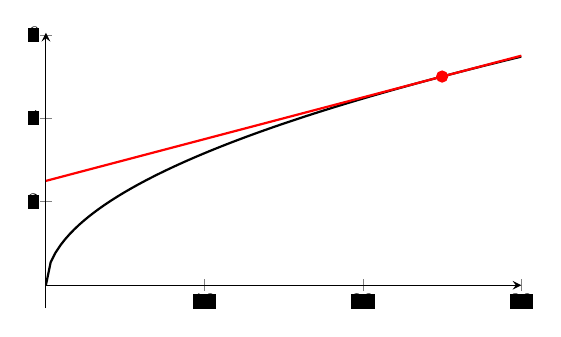
\begin{tikzpicture}
        \begin{axis}[height=2in]
          \addplot[domain=0:30] {sqrt(x)};
          \addplot[red, domain=0:30] {0.1*(x-25)+5};
          \addplot[closed,red] coordinates {(25,5)};
        \end{axis}
      \end{tikzpicture}
    \end{solution}

  \item

    \note{Just a reminder that we can also do secant line approximation}

    \begin{problem}[\stretch{0.75}]
      What's another way you could approximate $\sqrt{22}$? Would that give you an upper bound or lower bound for the actual value of $\sqrt{22}$? 
    \end{problem}

    \begin{solution}
      We could also approximate $\sqrt{22}$ by finding the equation of a secant line
      between the points $(16, 4)$ and $(25, 5)$. This would give us a lower bound
      for the actual value.

      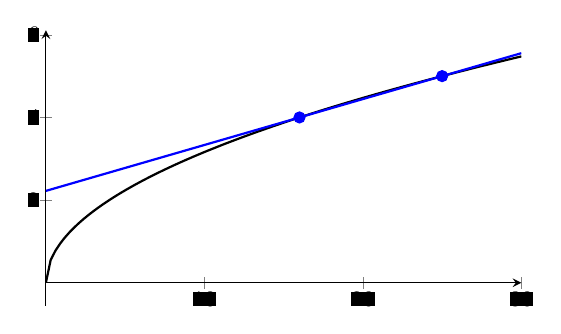
\begin{tikzpicture}
        \begin{axis}[height=2in]
          \addplot[domain=0:30] {sqrt(x)};
          \addplot[blue, domain=0:30] {(1/9)*(x-25)+5};
          \addplot[closed,blue] coordinates {(16,4) (25,5)};
        \end{axis}
      \end{tikzpicture}
    \end{solution}

  \item
    \begin{problem}[\nstretch{0.15}]
      What was the relevant function $f(x)$ in this problem?  What does
      the sign of $f''(x)$ have to do with your answer?
    \end{problem}

    \begin{solution}
        The relevant function was $f(x)=\sqrt{x}$. The sign of $f''(x)$ would tell
        us the concavity of $f$. We knew that our tangent line approximation was an
        overestimate because the graph of $y=\sqrt{x}$ is concave down.
    \end{solution}

  \end{enumerate}

\item 
  \begin{problem}[1in]
    In your Edfinity homework, you saw that the derivative of $f(x)^2$ is not $2 f(x)$. Now, we'll find a correct formula for the derivative of $f(x)^2$.

    Let $g(x) = f(x)^2$. Find $g'(x)$. (Which rule do you need to use?)
  \end{problem}

  \begin{solution}
    We should use the Product Rule, since $g(x) = f(x) \cdot f(x)$. 
    \begin{align*}
        g'(x) &= f'(x)f(x) + f(x)f'(x) \\
        &= 2f(x)f'(x).
    \end{align*}
  \end{solution}

\item  \label{graphing-worksheet-odd}

  We'd like to get an accurate graph of $f(x) = \dfrac{18 x^2 + 2}{x}$. Answer the questions below in whatever order makes most sense to you, and use them to sketch the graph of $f$.
  \begin{enumerate}

  \item
    \begin{problem}[\vfill]
      What is the domain of $f$? Does $f$ have any useful symmetry?
    \end{problem}

    \begin{solution}
      The domain of $f$ is $(-\infty, 0) \cup (0, \infty)$. We know that $f$ is odd, since
      \begin{align*}
        f(-x) &= \frac{18(-x)^2 + 2}{-x} \\
        &= -\frac{18x^2 + 2}{x} \\
        &= -f(x).
      \end{align*}
    \end{solution}

  \item
    \begin{problem}[\stretch{0.75}]
      Can you find the $x$- and $y$-intercepts of $f$?
    \end{problem}

    \begin{solution}
      There is no $y$-intercept, since $f(0)$ is undefined. There are no $x$-intercepts,
      since $f(x)=0$ has no real solutions.
    \end{solution}

  \item
    \begin{problem}[\vfill]
      Find and classify all discontinuities of $f$. Justify your classifications using limits. If a limit does not exist, find both one-sided limits. 
    \end{problem}

    \begin{solution}
      Since $f$ is defined by a single algebraic formula, the only discontinuity is at
      $x=0$. Let's consider the limit as $x \to 0$. Direct substitution gives us 
      $\frac{2}{0}$, which suggests that we have a vertical asymptote and should
      consider the one-sided limits.
      \begin{itemize}
        \item $\displaystyle \lim_{x \to 0^-} \frac{18x^2+2}{x} = -\infty$ since
        the numerator is positive and the denominator is negative when $x<0$. 
        \item $\displaystyle \lim_{x \to 0^+} \frac{18x^2+2}{x} = \infty$ since
        the numerator is positive and the denominator is positive when $x>0$. 
      \end{itemize}
      Since at least one one-sided limit is $\pm \infty$, $x=0$ is a vertical asymptote.
    \end{solution}

  \item
    \begin{problem}[\nstretch{0.75}]
      Find all horizontal asymptotes of $f$.
    \end{problem}

    \begin{solution}
      We need to consider the limits as $x$ goes to $\pm \infty$. We consider
      the dominant terms in the numerator and denominator.
      \begin{itemize}
        \item $\displaystyle \lim_{x \to -\infty} \frac{18x^2+2}{x} =
        \lim_{x \to -\infty} \frac{18x^2}{x} = \lim_{x \to -\infty} 18x = -\infty$.
        \item $\displaystyle \lim_{x \to \infty} \frac{18x^2+2}{x} =
        \lim_{x \to \infty} \frac{18x^2}{x} = \lim_{x \to \infty} 18x = \infty$.
      \end{itemize}
      These limits indicate that $f$ has no horizontal asymptotes.
    \end{solution}

  \item
    \begin{problem}[\vfill]
      On what intervals is $f(x)$ increasing? On what intervals is it decreasing?
    \end{problem}

    \begin{solution}
      First, we should find $f'(x)$. We can do this by rewriting $f(x)$ as $18x + 2x^{-1}$
      and then using the Power Rule: $f'(x) = 18 -2x^{-2}$. 
      
      Now we need to construct a sign
      chart for $f'(x)$. To do this, we should determine where $f'(x)$ is undefined or zero.
      We know that $f'(0)$ is undefined, and we can solve for the zeros as follows.
      \begin{align*}
        18 - \frac{2}{x^2} &= 0 \\
        18 &= \frac{2}{x^2} \\
        18x^2 &= 2 \\
        x^2 &= \frac{1}{9} \\
        x &= \pm \frac{1}{3}.
      \end{align*}
      These $x$-values will go on our sign chart, and we can test points to determine
      the sign of $f'(x)$ on each interval.
      \begin{center}
        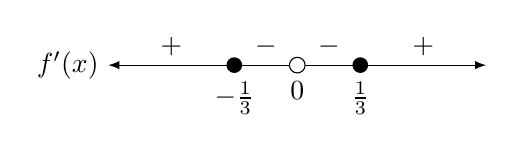
\begin{tikzpicture}[scale=0.8]
          \draw[<->] (-3,0) -- (3, 0);
          \node[left] at (-3,0) {$f'(x)$};
          \draw[shift={(-1,0)},color=black] (0pt,3pt) -- (0pt,-3pt) node[below] 
          {$-\frac{1}{3}$};
          \draw[shift={(0,0)},color=black] (0pt,3pt) -- (0pt,-3pt) node[below] {$0$};
          \draw[shift={(1,0)},color=black] (0pt,3pt) -- (0pt,-3pt) node[below] 
          {$\frac{1}{3}$};
          \node[circle, fill=black, inner sep=2pt] at (-1,0) {};
          \node[circle, draw=black, fill=white, inner sep=2pt] at (0,0) {};
          \node[circle, fill=black, inner sep=2pt] at (1,0) {};
          \node[above] at (-2,0) {$+$};
          \node[above] at (-0.5,0) {$-$};
          \node[above] at (2,0) {$+$};
          \node[above] at (0.5,0) {$-$};
        \end{tikzpicture}
      \end{center}

      This means that $f$ is increasing on the intervals $(-\infty, -\frac{1}{3})$ and
      $(\frac{1}{3}, \infty)$, decreasing on the intervals $(-\frac{1}{3},0)$ and 
      $(0, \frac{1}{3})$.
    \end{solution}

  \item
    \begin{problem}[\vfill]
      On what intervals is $f(x)$ concave up? On what intervals is it concave down?
    \end{problem}

    \begin{solution}
      First, we should find $f''(x)$ by taking the derivative of $f'(x) = 18 -2x^{-2}$.
      Using the Power Rule gives us $f''(x) = 4x^{-3}$.

      Now we need to make a sign chart for $f''(x)$. Again, $f''(x)$ is undefined at 
      $x=0$. There are no $x$-values for which $f''(x)$ is zero. Testing points to determine
      the sign of $f''(x)$ in each interval gives us the following sign chart.
      \begin{center}
        \begin{tikzpicture}[scale=0.8]
          \draw[<->] (-3,0) -- (3, 0);
          \node[left] at (-3,0) {$f''(x)$};
          \draw[shift={(0,0)},color=black] (0pt,3pt) -- (0pt,-3pt) node[below] {$0$};
          \node[circle, draw=black, fill=white, inner sep=2pt] at (0,0) {};
          \node[above] at (-1.5,0) {$-$};
          \node[above] at (1.5,0) {$+$};
        \end{tikzpicture}
      \end{center}
      This means $f$ is concave down on the interval $(-\infty, 0)$ and
      concave up on the interval $(0, \infty)$. 
    \end{solution}

  \item

    \note{Although concavity changes at $x = 0$, there isn't an inflection point there because $f$ is undefined at $0$.}

    \begin{problem}[0.5in]
      What are the turning points of $f$? The inflection points of $f$?
    \end{problem}

    \begin{solution}
      There are turning points at $x=-\frac{1}{3}$ and $x=\frac{1}{3}$, because $f$
      changes from increasing to decreasing or vice versa. There are no inflection points.
      Although $f$ changes from concave down to concave up at $x=0$, this is because
      we have a vertical asymptote, not an inflection point.
    \end{solution}

  \item
    \begin{problem}[\vfill]
      Sketch a rough graph of $f(x)$ that incorporates all of the above
      information.
    \end{problem}

    \begin{solution}
      \begin{center}
        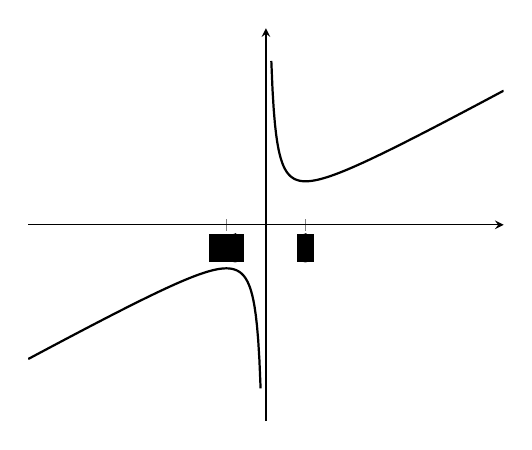
\begin{tikzpicture}
          \begin{axis}[restrict y to domain=-50:50, ytick=\empty, samples=400,
          xtick={-1/3, 1/3}, xticklabels={$-\frac{1}{3}$, $\frac{1}{3}$}]
            \addplot[domain=-2:2]{(18*x^2 + 2)/x};
          \end{axis}
        \end{tikzpicture}
      \end{center}
    \end{solution}

  \end{enumerate}

\end{enumerate}
\end{document}
